\chapter{Bound States from Exchange Amplitudes}
\label{ch:volume-ii-bound-states-exchange}
\ConventionsLorentzian


\section{Exchange Model}

Consider two real scalar fields in four spacetime dimensions with Lorentzian
Lagrangian density
\[
  \mathcal L
  =
  -\frac12\partial_\mu\phi_1\partial^\mu\phi_1
  -\frac12m_1^2\phi_1^2
  -\frac12\partial_\mu\phi_2\partial^\mu\phi_2
  -\frac12m_2^2\phi_2^2
  -\frac12g\phi_1^2\phi_2 .
\]
The masses \(m_1,m_2\) are positive, and \(g\) is a real coupling. Use the
same mostly-plus convention as before. The scalar propagators and cubic
vertex are
\[
  \phi_i:\quad
  \frac{-\ii}{k^2+m_i^2-\ii0},
  \qquad
	  \phi_1\phi_1\phi_2:\quad -\ii g .
\]
This Lagrangian is used as a perturbative exchange model in the sense of
Section~\ref{sec:volume-ii-scalar-model-status}.  The pole criterion derived
below is a statement about any exact massive local theory whose amplitude has
the displayed analytic structure; the polynomial scalar density by itself is
only the finite-cutoff or effective description from which the tree kernel is
computed.

The connected \(\phi_1\phi_1\to\phi_1\phi_1\) tree amplitude receives
\(s\)-, \(t\)-, and \(u\)-channel exchange contributions:
\[
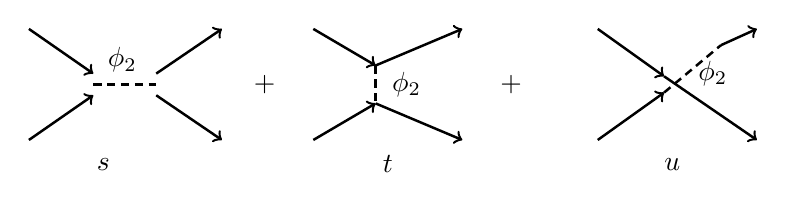
\begin{tikzpicture}[baseline=-0.5ex,scale=0.86,
  one/.style={line width=0.9pt},
  two/.style={dash pattern=on 3pt off 2pt,line width=0.9pt}]
  \begin{scope}[xshift=-4.2cm]
    \draw[one,->] (-1.1,0.82)--(-0.15,0.16);
    \draw[one,->] (-1.1,-0.82)--(-0.15,-0.16);
    \draw[two] (-0.15,0)--(0.78,0);
    \draw[one,->] (0.78,0.16)--(1.75,0.82);
    \draw[one,->] (0.78,-0.16)--(1.75,-0.82);
    \node at (0.28,0.36) {\(\phi_2\)};
    \node at (0,-1.18) {\(s\)};
  \end{scope}
  \node at (-1.82,0) {\(+\)};
  \begin{scope}
    \draw[one,->] (-1.1,0.82)--(-0.18,0.28);
    \draw[one,->] (-0.18,0.28)--(1.1,0.82);
    \draw[one,->] (-1.1,-0.82)--(-0.18,-0.28);
    \draw[one,->] (-0.18,-0.28)--(1.1,-0.82);
    \draw[two] (-0.18,0.28)--(-0.18,-0.28);
    \node[right] at (-0.08,0) {\(\phi_2\)};
    \node at (0,-1.18) {\(t\)};
  \end{scope}
  \node at (1.82,0) {\(+\)};
  \begin{scope}[xshift=4.2cm]
    \draw[one,->] (-1.1,0.82)--(-0.12,0.12);
    \draw[one,->] (-1.1,-0.82)--(-0.12,-0.12);
    \draw[two] (-0.12,-0.12)--(0.72,0.58);
    \draw[one,->] (-0.12,0.12)--(1.25,-0.82);
    \draw[one,->] (0.72,0.58)--(1.25,0.82);
    \node at (0.6,0.16) {\(\phi_2\)};
    \node at (0,-1.18) {\(u\)};
  \end{scope}
\end{tikzpicture}
\]
With all external momenta on the \(\phi_1\) mass shell, define
\[
  s=-(k_1+k_2)^2,\qquad
  t=-(k_1-k_3)^2,\qquad
  u=-(k_1-k_4)^2 .
\]
Here the metric is mostly plus, \(k_i^2=-m_1^2\), \(k_1,k_2\) are incoming,
and \(k_3,k_4\) are outgoing.  Momentum conservation gives the Mandelstam
constraint
\[
  s+t+u=4m_1^2 .
\]
The tree-level invariant amplitude is
\[
  \mathcal M_{\mathrm{tree}}(s,t,u)
  =
  g^2
  \left(
    \frac{1}{m_2^2-s-\ii0}
    +
    \frac{1}{m_2^2-t-\ii0}
    +
    \frac{1}{m_2^2-u-\ii0}
  \right).
\]

In the center-of-mass frame for equal incoming masses \(m_1\),
\[
  s=E^2,
  \qquad
  t=-\frac{E^2-4m_1^2}{2}(1-z),
  \qquad
  u=-\frac{E^2-4m_1^2}{2}(1+z),
\]
where \(E\) is the total energy and \(z=\cos\theta\). The two-\(\phi_1\)
threshold is
\[
  s=4m_1^2 .
\]

\section{Pole Below a Two-Particle Threshold}

Assume
\[
  0<m_2<2m_1 .
\]
Then the \(s\)-channel pole \(s=m_2^2\) lies below the two-\(\phi_1\)
threshold. It is outside the physical two-\(\phi_1\) scattering region
\(s\ge4m_1^2\), but it is reached by analytic continuation in the invariant
energy variable.

\begin{center}
\begin{tikzpicture}[>=Stealth,scale=0.95]
  \draw[->,line width=0.75pt] (-0.4,0)--(7.4,0) node[right] {$s$};
  \draw[->,line width=0.75pt] (0,-1.35)--(0,2.05)
    node[above] {$\operatorname{Im}s$};
  \fill[blue!80!black] (2.1,0) circle (2.6pt);
  \node[blue!80!black,below] at (2.1,-0.16) {$m_2^2$};
  \draw[red!75!black,line width=2.0pt] (4.6,0)--(7.05,0);
  \node[red!75!black,below] at (4.6,-0.18) {$4m_1^2$};
  \node[blue!80!black,align=center] at (1.65,1.18)
    {stable\\pole};
  \draw[blue!80!black,->,line width=0.75pt] (1.78,0.82)--(2.04,0.12);
  \node[red!75!black,align=center] at (5.95,0.78)
    {two-particle\\cut};
  \draw[decorate,decoration={brace,amplitude=5pt},gray!70]
    (2.22,0.48)--(4.45,0.48);
  \node[gray!70!black] at (3.35,0.85) {gap};
\end{tikzpicture}
\end{center}

The scattering conclusion is precise: the two-\(\phi_1\) channel couples to a
stable one-particle state of invariant mass \(m_2\). In the present model that
state is represented explicitly by the field \(\phi_2\). In a theory where no
elementary field for that state is introduced, the same below-threshold pole
is the scattering signature of a stable bound state. The pole criterion and
the microscopic origin of the state are separate statements.

\begin{remark}[Existence is dynamical input]
The exchange model above contains the state at \(s=m_2^2\) because the
Lagrangian already contains the stable field \(\phi_2\) and the chosen masses
place its pole below the two-\(\phi_1\) threshold.  In a theory without such an
elementary field, the existence of a below-threshold composite pole is a
nonperturbative fact about the spectrum and the connected four-point function,
requiring dynamical spectral input beyond locality, unitarity, and the local
action.  The rest of this chapter uses the conditional statement: if an isolated
stable pole is present in a two-particle channel, then its position, spin, and
factorized residue have the scattering consequences derived below.
\end{remark}

Near a stable pole, the connected amplitude factorizes. If \(B\) denotes the
one-particle state and \(P=k_1+k_2\), then
\[
  \mathcal M(s,z)
  \sim
  \frac{\Gamma_{\mathrm{out}}(z)\Gamma_{\mathrm{in}}(z)}
       {M_B^2-s-\ii0}
  +\text{terms regular at }s=M_B^2 ,
\]
where \(M_B\) is the bound-state mass. The functions
\(\Gamma_{\mathrm{in}}\) and \(\Gamma_{\mathrm{out}}\) are channel couplings;
they are determined by matrix elements between the one-particle state \(B\)
and two-particle states created by local or composite operators.

\section{One-Dimensional Pole Criterion as Orientation}
\label{sec:bound-state-one-dimensional-orientation}

The elementary one-dimensional Schr\"odinger model is useful here only as an
orientation for the bound-state pole criterion.  Its Hilbert-space conventions
belong to the general discussion of continuous spectra in
Section~\ref{sec:rigged-hilbert-continuous-spectrum}, and its unitary
Schr\"odinger evolution is part of the quantum-mechanical setup of
Chapter~\ref{ch:hamiltonian-evolution-time-sliced-path-integrals}.  The
detailed one-dimensional analytic continuation, including outgoing resonance
poles and the two-sheeted energy plane, is treated in
Section~\ref{sec:resonance-one-dimensional-outgoing-poles}.

For the present stable-bound-state purpose, take a short-range Hamiltonian
\[
  H=-\frac{1}{2\mu}\frac{\dd^2}{\dd x^2}+V(x),
  \qquad
  E_{\mathrm{nr}}=\frac{k^2}{2\mu},
\]
with \(V\) real.  After fixing the real-\(k\) scattering normalization, an
outgoing solution has the asymptotic form
\[
  \psi_k^{\mathrm{out}}(x)
  \sim
  S(k)^{-1}\ee^{-\ii kx}+\ee^{\ii kx}
  \qquad (x\to+\infty).
\]
Analytic continuation to \(k=\ii\alpha\), \(\alpha>0\), gives
\[
  \psi_{\ii\alpha}^{\mathrm{out}}(x)
  \sim
  S(\ii\alpha)^{-1}\ee^{\alpha x}
  +
  \ee^{-\alpha x}.
\]
An \(L^2\) bound-state wave function cannot contain the growing term
\(\ee^{\alpha x}\).  Thus normalizability requires
\[
  S(\ii\alpha)^{-1}=0,
  \qquad
  E_{\mathrm{nr}}=-\frac{\alpha^2}{2\mu},
\]
or equivalently a pole of \(S(k)\) at \(k=\ii\alpha\) on the positive imaginary
\(k\)-axis.  In the relativistic amplitude this statement becomes: a stable
bound state below a two-particle threshold appears as a first-sheet pole below
the corresponding branch cut, with the sheet convention of
Section~\ref{sec:physical-region-and-first-sheet}.

\section{Partial Waves}

For an equal-mass scalar elastic channel in four dimensions, write
\[
  z=\cos\theta,
  \qquad
  s=E^2 .
\]
The underlying partial waves are generalized two-particle asymptotic states.
In the center-of-mass frame, with the \(\delta\)-normalized sharp-momentum
basis,
\[
  \langle \vec k_1,\vec k_2
  |E,\vec P=\vec0,\ell,m_\ell\rangle_\delta
  =
  \delta^{(3)}(\vec k_1+\vec k_2)\,
  \delta(\omega_1+\omega_2-E)\,
  \mathcal N(E)Y_{\ell m_\ell}(\widehat k_1),
\]
where
\[
  \omega_i=\sqrt{|\vec k_i|^2+m^2},
  \qquad
  |\vec k_1|=|\vec k_2|=k,
  \qquad
  E=2\sqrt{k^2+m^2}.
\]
For identical scalar bosons,
\[
  \mathcal N(E)
  =
  \left(\frac{2E}{k\,\omega_1\omega_2}\right)^{1/2},
  \qquad
  \ell\in2\mathbb Z_{\ge0}.
\]
For a distinguishable equal-mass pair, such as a charged scalar and its
antiparticle, the factor of \(2\) under the square root is absent and both
even and odd \(\ell\) occur. The ordered-particle invariant amplitude below
uses the \(16\pi\) normalization fixed in
Chapter~\ref{ch:cross-sections-unitarity}; for an unordered identical-boson
channel, the same physical information is obtained after Bose symmetrization
and restriction to even partial waves, with the \(32\pi\) normalization in
Equation~\eqref{eq:identical-partial-wave-conversion}.

Rotational invariance diagonalizes the elastic single-channel matrix element,
\begin{equation}
  |E,\ell,m_\ell\rangle^{\mathrm{in}}
  =
  S_\ell(E)|E,\ell,m_\ell\rangle^{\mathrm{out}}
  \quad
  \text{in the elastic sector}.
  \label{eq:exchange-elastic-partial-wave-s-matrix}
\end{equation}
When additional channels with the same conserved quantum numbers are open,
Equation~\eqref{eq:exchange-elastic-partial-wave-s-matrix} is the elastic
component of a larger unitary matrix and gives \(|S_\ell(E)|\le1\).

In the elastic region, define partial-wave amplitudes by
\begin{equation}
  \mathcal M(s,z)
  =
  16\pi\sum_{\ell=0}^{\infty}
  (2\ell+1)\mathcal M_\ell(s)P_\ell(z),
  \label{eq:exchange-partial-wave-expansion}
\end{equation}
equivalently
\begin{equation}
  \mathcal M_\ell(s)
  =
  \frac{1}{32\pi}\int_{-1}^{1}\dd z\,
  P_\ell(z)\mathcal M(s,z).
  \label{eq:exchange-partial-wave-projection}
\end{equation}
The elastic partial-wave \(S\)-matrix eigenvalue is written
\[
  S_\ell(s)=1+2\ii\,\rho(s)\mathcal M_\ell(s),
  \qquad
  \rho(s)=\sqrt{1-\frac{4m^2}{s}},
\]
with the branch chosen by \(\rho(s)>0\) for \(s>4m^2\). Elastic unitarity is
\[
  |S_\ell(s)|=1
\]
on the physical elastic interval.

A stable spin-\(\ell\) state of mass \(M_B<2m\) coupled to the two-particle
channel gives
\[
  \mathcal M_\ell(s)
  =
  \frac{r_\ell}{M_B^2-s}
  +\text{regular terms},
\]
where the residue \(r_\ell\) is determined by the squared coupling of the
state to the two-particle channel with angular momentum \(\ell\).

\begin{center}
\begin{tikzpicture}[>=Stealth,scale=0.95]
  \draw[->,line width=0.75pt] (-0.3,0)--(7.2,0) node[right] {$s$};
  \draw[->,line width=0.75pt] (0,-1.2)--(0,2.05)
    node[above] {\(\operatorname{Im}s\)};
  \draw[red!75!black,line width=2.0pt] (4.75,0)--(6.85,0);
  \node[red!75!black,below] at (4.75,-0.16) {$4m^2$};
  \fill[blue!75!black] (2.55,0) circle (2.5pt);
  \node[blue!75!black,below] at (2.55,-0.16) {$M_B^2$};
  \node[blue!75!black,align=center] at (2.45,1.05)
    {pole in\\\(\mathcal M_\ell\)};
  \node[red!75!black,align=center] at (5.85,0.82)
    {elastic\\cut};
  \draw[blue!75!black,->,line width=0.8pt] (2.45,0.72)--(2.55,0.12);
\end{tikzpicture}
\end{center}

For the exchange model, the \(s\)-channel term is independent of \(z\). Its
below-threshold pole therefore appears in the \(\ell=0\) partial wave. Higher
spin bound states arise when the pole residue has the angular dependence of
\(P_\ell(z)\), or more generally the corresponding spin-\(\ell\) tensor
structure.

The spin carried by a channel pole can be read directly from this angular
dependence. As an algebraic illustration, consider the numerator structure of
scalar QED, developed later in the gauge-theory chapters; here only the
Lorentz-contracted photon-exchange numerator is used, not the full gauge theory.
The charged scalar-antiscalar annihilation channel has an \(s\)-channel
exchange numerator proportional to
\[
  (p_1-p_2)^\mu(p_3-p_4)_\mu .
\]
In the center-of-mass frame this numerator is
\[
  4k^2\cos\theta
  =
  4k^2P_1(\cos\theta),
\]
up to the overall sign fixed by momentum routing and metric conventions. The
massless pole is therefore an \(\ell=1\) pole in this channel. The invariant
statement is the pole position and spin-one residue in the scalar-antiscalar
scattering amplitude; the microscopic description of the corresponding
one-particle state is additional data of the theory.

\section{Operator Interpretation}

Let \(O_B(x)\) be a local or suitably smeared composite operator with nonzero
overlap with a stable state \(B\),
\[
  \bra{\vac}O_B(0)|B(P)\rangle\ne0,
  \qquad
  P^2=-M_B^2 .
\]
Then the spectral representation of a two-point function of \(O_B\) contains
an atom at \(M_B^2\). The same state appears in four-point functions through a
factorizing pole. For external operators \(O_1,O_2,O_3,O_4\), and
\(P\) the momentum flowing through the channel,
\[
  \widetilde G_4(P;\cdots)
  \sim
  \frac{
    \bra{\vac}O_3O_4|B(P)\rangle
    \langle B(P)|O_1O_2\ket{\vac}}
       {P^2+M_B^2-\ii0}
  +\text{regular terms}.
\]
After LSZ reduction on the external stable particles, this factorization
becomes the bound-state pole of the scattering amplitude.

The particle content of a theory is therefore read from spectral and
asymptotic data. A field appearing in a Lagrangian can interpolate a stable
state, and a composite operator can interpolate a stable state. The analytic
pole and its residue state the channel coupling; additional structural data
state how the corresponding state is represented inside the theory.
